\documentclass{beamer}
\title{Cascade control}
\author{Fred-Olav}
\begin{document}
\maketitle

\begin{frame}
	\frametitle{Enkelt reguleringssystem}

	
$$\includegraphics[width=0.8\textwidth]{cont05.eps}$$

\end{frame}





\begin{frame}
	\frametitle{Kaskadekoblet reguleringssystem}

	
$$\includegraphics{cont14.eps}$$

\end{frame}





%A very common example of cascade control is a \textit{valve positioner}, which receives a command signal from a regular process controller, and in turn works to ensure the valve stem position precisely matches that command signal.  The control valve's stem position is the process variable (PV) for the positioner, just as the command signal is the positioner's setpoint (SP).  Valve positioners therefore act as ``slave'' controllers to ``master'' process controllers controlling pressure, temperature, flow, or some other process variable.

%The purpose of cascade control is to achieve greater stability of the primary process variable by regulating a secondary process variable in accordance with the needs of the first.  An essential requirement of cascaded control is that the secondary process variable be faster-responding (i.e. shorter lag and dead times) than the primary process variable. 

%An analogy for understanding cascade control is that of \textit{delegation} in a work environment.  If a supervisor delegates some task to a subordinate, and that subordinate performs the task without further need of guidance or assistance from the supervisor, the supervisor's job is made easier.  The subordinate takes care of all the little details that would otherwise burden the supervisor if the supervisor had no one to delegate to.  This analogy also makes it clear why the secondary process variable must be faster-responding than the primary process variable: the supervisor-subordinate management structure fails to work if the supervisor does not maintain focus on long-term goals (i.e. longer-term than the completion time of the tasks given to subordinates).  If a supervisor focuses on achieving goals that are shorter-term than the time required for subordinates to complete their assignments, the supervisor will inevitably call for ``course changes'' that are too quick for the subordinates to execute.  This will lead to the subordinates ``lagging'' behind the supervisor's orders, to the detriment of everyone's satisfaction.

%\vskip 10pt

%\filbreak

%An example of cascade control applied to a real industrial process is shown here, for a \textit{dryer} system where heated air is used to evaporate water from a granular solid.  The primary process variable is the outlet air exiting the dryer, which should be maintained at a high enough temperature to ensure water will not remain in the upper layers of the solid material.  This outlet temperature is fairly slow to react, as the solid material mass creates a large lag time:
\begin{frame}
	\frametitle{Eksempel på kaskadekoblet reguleringsystem}

	
$$\includegraphics{cont16.eps}$$

\end{frame}



%There are several parameters influencing the temperature of the outlet air other than the moisture content of the drying material.  These include air flow, ambient air temperature, and variations in steam temperature.  Each one of these variables is a \textit{load} on the process variable we are trying to control (outlet air temperature).  If any of these parameters were to suddenly change, the effect would be slow to register at the outlet temperature even though there would be immediate impact at the bottom of the dryer where the heated air enters.  Correspondingly, the control system would be slow to correct for any of these changing loads.

%\filbreak

%We may better compensate for these loads by installing a second temperature transmitter at the inlet duct of the dryer, with its own controller to adjust steam flow at the command of the primary controller:

%$$\includegraphics{cont15.eps}$$

%Now, if any of the loads related to incoming air flow or temperature vary, the secondary controller (TC-1b) will \textit{immediately} sense the change in dryer inlet temperature and compensate by adjusting steam flow through the heat exchanger.  Thus, the ``slave'' control loop (1b) helps stabilize the ``master'' control loop (1a) by reacting to load changes long before any effect might manifest at the dryer outlet.

%A helpful way to think of this is to consider the slave controller as \textit{shielding} the master controller from the loads previously mentioned (incoming air flow, ambient temperature, and steam temperature).  Of course, these variables still act as loads to the slave controller, as it must continuously adjust the steam valve to compensate for changes in air flow, ambient air temperature, and steam temperature.  However, so long as the slave controller does a good job of stabilizing the air temperature entering the dryer, the master controller will never ``see'' the effects of those load changes.  Responsibility for incoming air temperature has been delegated to the slave controller, and as a result the master controller is conveniently isolated from the loads impacting that loop.

%To re-emphasize an important point, one of the non-negotiable requirements for cascade control is that the secondary (slave) loop must be \textit{faster-responding} than the primary (master) loop.  Cascade control cannot function if this speed relationship is reversed.  Temperature controller TC-1b is able to be a slave to controller TC-1a because the natural response time of the temperature at the dryer's bottom is much shorter than at the dryer's top with respect to any changes in steam valve position.

%\vskip 10pt

%\filbreak

%A common implementation of cascade control is where a flow controller receives a setpoint from some other process controller (pressure, temperature, level, analytical, etc.), fluid flow being one of the fastest-responding process types in existence.  A feedwater control system for a steam boiler -- shown here in pneumatic form -- is a good example: 

%$$\includegraphics{cont19.eps}$$

%The ``secondary'' or ``slave'' flow controller works to maintain feedwater flow to the boiler at whatever flow rate is desired by the level controller.  If feedwater pressure happens to increase or decrease, any resulting changes in flow will be quickly countered by the flow controller without the level controller having to react to a consequent upset in steam drum water level.  Thus, cascade control works to guard against steam drum level instability resulting from changes in the feedwater flow caused by factors outside the boiler.  As stated previously, the slave (flow) controller effectively \textit{shields} the master (level) controller from loads in the feedwater supply system, so that master controller doesn't have to deal with those loads.

%This level/flow cascade control system also embodies the principle of the secondary (slave) loop being faster-responding than the primary (master) loop.  Water flow is an inherently fast process, the flow rate responding immediately to changes in valve position.  By contrast, water level is a much slower-responding type of process.  If you perform a ``thought experiment'' where the feedwater valve is suddenly opened fully, it is easy to see that the feedwater flow rate will immediately reach its full (100\%) value while the steam drum's water level will merely begin to rise, taking time to reach its full (100\%) value.

%\filbreak

%It is worth noting that the inclusion of a flow control ``slave'' loop to this boiler water level control system also helps to overcome a potential problem of the control valve: nonlinear behavior.  In the control valves chapter, we explore the phenomenon of \textit{installed valve characteristics} (Section \ref{installed_valve_characteristic} beginning on page \pageref{installed_valve_characteristic}), specifically noting how changes in pressure drop across a control valve influences its throttling behavior.  The result of these pressure changes is a non-linearization of valve response, such that the valve tends to be more responsive near its closed position and less responsive near its open position.  One of the benefits of cascaded flow control is that this problem becomes confined to the secondary (flow control) loop, and is effectively removed from the primary control loop.  To phrase it simply, distorted valve response becomes ``the flow controller's problem'' rather than something the level controller must manage.  The result is a level control system with more predictable response.  \index{Installed valve characteristic} 

%\vskip 10pt

%\filbreak

%A classic example of cascade control strategy is found in \textit{motion control} applications, where an electric motor is used as the final control element to precisely position a piece of machinery.  In this capacity, the motor is usually called a \textit{servo}.  Robotic systems make extensive use of servo motors and cascaded control loops to modulate power to those motors.  The following illustration shows a triple-cascade control system\footnote{Interestingly, servo motor control is one application where \textit{analog} loop controllers have historically been favored over digital loop controllers, simply for their superior speed.  An opamp-based P, PI, or PID controller is lightning-fast because it has no need to digitize any analog process variables (analog-to-digital conversion) nor does it require time for a clock to sequence step-by-step through a written program as a microprocessor does.  Servomechanism processes are inherently fast-responding, and so the controller(s) used to control servos must be faster yet.} for a motor-actuated elevator, precisely controlling the position of the elevator through cascaded velocity and motor current control:  \index{Motion control system}  \index{Triple-cascaded loops}  \index{Servo motor control}

%$$\includegraphics{cont75.eps}$$

%Hypothetically, the position of the elevator could be controlled with a single PID controller sensing platform position and directly sending power to the motor.  However, much more precise control of the platform is achievable by sensing position, velocity, and motor current, and controlling each one of those variables with its own loop.  In motion control systems, each successive variable is the time-derivative of its precursor.  Velocity, for instance, is the time-derivative of position ($v = {dx \over dt}$).  Motor current, which is usually proportional to motor torque, which in turn is proportional to the angular acceleration ($\alpha$) of the winch and consequently the linear acceleration of the platform ($a$), is the time-derivative of velocity ($a = {dv \over dt}$).  If it were not for cascading, a single PID controller would have to control position by manipulating the \textit{acceleration} of the platform (i.e. motor current).  This would make the process characteristic ``runaway'' in nature, as any fixed amount of current will cause the platform to accelerate\footnote{At one specific current level, the motor will develop just enough torque to hold the platform's weight, at which point the acceleration will be zero.  Any amount of current above this value will cause an upward acceleration, while any amount of current below this value will cause a downward acceleration.}.

%Here with servomechanisms we see how cascading not only has the effect of ``shielding'' certain load variables from the master controller's view, but it also simplifies the dynamic characteristics of the process from that same point of view.  Instead of the position controller having to regulate an inherently ``runaway'' process, it now sees the process as having an ``integrating'' characteristic, since any constant output signal from the position controller results in the platform holding to a constant velocity (i.e. platform position will change at a constant rate over time, rather than at an accelerating rate).

%\vskip 10pt

%A necessary step in implementing cascade control is to ensure the secondary (``slave'') controller is well-tuned \textit{before} any attempt is made to tune the primary (``master'') controller.  Just a moment's thought is all that is needed to understand why this precedence in tuning must be: it is a simple matter of dependence.  The slave controller does not depend on good tuning in the master controller in order to control the slave loop.  If the master controller were placed in manual (effectively turning off its automatic response), the slave controller would simply control to a constant setpoint.  However, the master controller most definitely depends on the slave controller being well-tuned in order to fulfill the master's ``expectations.''  If the slave controller were placed in manual mode, the master controller would not be able to exert any control over its process variable whatsoever.  Clearly then, the slave controller's response is essential to the master controller being able to control its process variable, therefore the slave controller should be tuned first when initially commissioning or optimizing a cascade control system.

%\vskip 10pt

%Just like supervisory control systems where a process controller receives a ``remote'' setpoint signal from some other system, the secondary (``slave'') controller in a cascade system typically has three different operating modes:

%\begin{itemize}
%\item \textbf{Manual mode:} Controller takes no automatic action.  Output value set by human operator.
%\item \textbf{Automatic mode:} Controller automatically adjusts its output to try to keep PV = SP.  Setpoint value set ``locally'' by human operator.
%\item \textbf{Cascade mode:} Controller automatically adjusts its output to try to keep PV = SP.  Setpoint value set ``remotely'' by primary (master) controller.
%\end{itemize}
%
%This means it is possible to defeat a cascade control system by placing the secondary controller in the wrong mode (automatic) just as it is possible to defeat any control system by placing the controller in manual mode.  If a controller is ``slaved'' to another controller, it must be left in \textit{cascade} mode in order for the control strategy to function as designed.

%% ADD: discuss how cascaded flow systems may result in shifting the characteristics of a process from self-regulating (with lag) to purely integrating.

\end{document}
